% ---------------------------------------------------------------------
% ---------------------------------------------------------------------
% ---------------------------------------------------------------------

\chapter[Introduction]{Introduction}
\label{chap:intro}

Networks are fundamental in many fields of science as they provide a powerful way to model complex systems and relationships between entities at different scales. By representing entities as nodes and connections between them as edges, networks can help researchers understand how information, energy, materials, and other resources flow through a system, identify patterns and structures within the data, and make predictions about system behavior. Many real life problems can be modeled as graphs or discretized as networks and that is why they are widely used in many fields such as physics, biology, sociology, statistics, or computer science amomg others. Network analysis in all these areas have led to significant advances in our understanding of the world around us \cite{albert2002statistical, katz1953new, newman2018networks}.

\section{Mathematical notation}
\label{sec:graph}
This section introduces a brief review of the definitions and notation pertaining to graphs, as well as some of their matrix representations, that will be used later in this study.

A network in the mathematical literature is, in its simplest form, a collection of interconnected nodes or vertices that represent entities, and the connections or edges between these nodes that represent relationships or interactions between the entities \cite{arrigo2022dynamic}.

\begin{definition}
    A network, or graph, is an ordered triple of sets $G = (V, E, \omega)$, where $V$ is the set of nodes, $E\subset V\times V$ is the set of edges among the nodes and $\omega$ is the set of  weights, also called values, strengths or costs, associated with each edge. A weighted graph is a graph in which each edge is given a numerical weight or cost. When all these weights are given the same weight (tipically, a value of $1$), then the graph, usually represented only by $G = (V, E)$, is called unweighted.
\end{definition}

The following two definitions that are central for this work are the concept of \textit{walk} and the \textit{adjacency matrix} of a graph.  

\begin{definition}
    A walk of length $w$ is a sequence of $w$ edges $(e_1, e_2, \dots, e_w)$ such that the target of $e_\ell$ coincides with the source of $e_{\ell+1}$ for all $\ell=1, 2, ..., w−1$.
\end{definition}
  
\begin{definition}
	Let $G =(V, E, \omega)$ be a weighted graph with $N$ nodes. Its adjacency matrix $\mathbf{A}\in\mathbb{R}^{N\times N}$ is entry-wise defined as
 
 \begin{equation}
  A_{ij} =
    \begin{cases}
      \omega_{ij} & \text{if there is an edge between nodes $i$ and $j$ with cost $\omega_{ij}$},\\
      0 & \text{otherwise},
    \end{cases}       
\end{equation}
for all $i, j = 1,2,\dots, N$.
\end{definition}

As a particular case, the adjacency matrix for unweighted graphs will have all their non-zero entries set to $A_{ij}=1$, indicating a connection between nodes $i$ and $j$.

Additionally, graphs are usually represented visually using a diagram (e.g., Figure \ref{fig:graphsv}), where nodes are represented as points and edges are represented as lines connecting the points. The direction of the edges allows us to divide graphs into \textit{directed} and \textit{undirected}. As a consequence of this, undirected graphs are represented by symmetric adjacency matrices, i.e., $A_{ij}=A_{ji}$ and, on the contrary, directed graphs by asymmetric matrices, $A_{ij}\ne A_{ji}$. The presence of loops, i.e., edges connecting a node to itself can also be indicated in this visual representation, $A_{ii} = 1$, in terms of the adjacency matrix.

\begin{figure}[h]\centering
	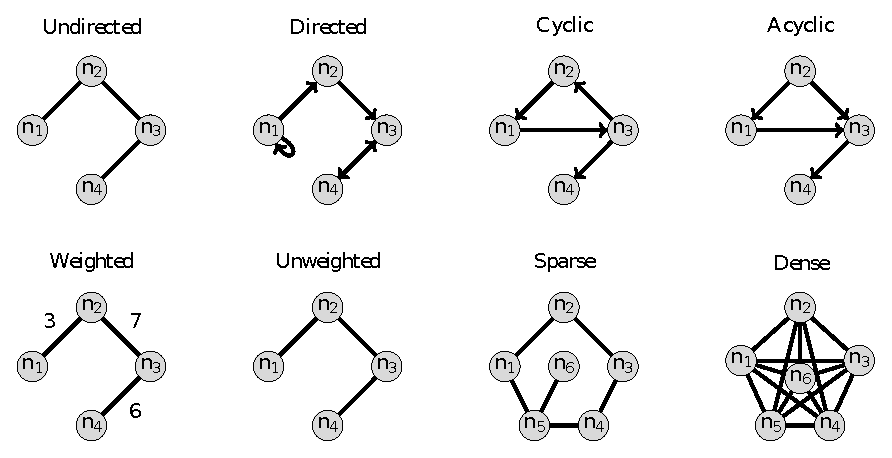
\includegraphics[width=0.75\textwidth]{graphsv}
	\caption{Examples of different network properties.}
	\label{fig:graphsv}
	\bigskip
\end{figure}

It is also worth mentioning other relevant network properties of graph theory for this work as:

\begin{itemize}
  \item \textit{Cyclic/acyclic networks}: Cyclic networks are networks where there is at least one path from a node to itself. In other words, they contain cycles or loops. Examples of cyclic networks include recurrent neural networks (RNNs) and feedback loops in control systems. On the other hand, acyclic networks are networks that do not contain any cycles so there is no path from any node back to itself. Examples of these networks are directed acyclic graphs (DAGs) as directed binary trees.
  \item \textit{Sparse/dense networks}: respectively, sparse/dense networks have a low/high density of connections between nodes compared to the total number of possible connections. Although there is a widespread agreement that most empirical networks are sparse, there is no formal definition of sparsity for any finite network, being the notion of "low" and "high" purely colloquial.
  \item \textit{Static/Dynamic networks}: A static network is a network that does not change over time. The relationships and connections between nodes are fixed and remain constant. On the contrary, a dynamic network is a network that changes over time. The relationships and connections between nodes can evolve and alter, resulting in a continually changing network structure.
\end{itemize}

Linear algebra will play a significant role in network analysis as graphs are represented by matrices. The analysis of networks often involves solving linear systems, determining eigenvalues and eigenvectors, and evaluating matrix functions. Moreover, the examination of dynamic processes on graphs will create systems of differential equations based on their structure. The behavior of the solution over time is expected to be highly impacted by the graph's structure (network topology), which is reflected in the spectral properties of the matrices related to the graph. This turns out to be one of the most basic questions about the network's structure; the identification of most relevant nodes within a network. This leads us to the concept of \textit{centrality}.

\section{Centrality measures}
\label{sec:centra}
 Centrality measures are metrics that are used to quantify the relative importance/influence/position of a node in a network. Indicators of centrality assign numbers or rankings, usually the higher the more important, to nodes within a graph corresponding to their network position based on different criteria. This gives rise to several types of centrality measures \cite{newman2018networks}:

\subsection*{Degree Centrality} The Degree Centrality measures the number of connections a node $i$ has to other nodes in the network. This is called the degree of a node ($k$). If we define $\mathbf{x}=(x_1,x_2,\dots,x_N)$ as the centrality vector of a graph with $N$ nodes, then 

\begin{equation}
    x_i^{(deg)}=k_i=\sum_{j=1}^{N}A_{ij}, ~~~i = 1,\dots, N.
\end{equation}
This measure is usually normalized by the maximal possible degree, $N − 1$, to obtain a number between 0 and 1. For certain networks, Degree Centrality can be very illuminating as it provides a straightforward and simple indication of a node's connectedness or level of popularity, but fails to consider other crucial elements of the network structure such as the importance of a node or its place within the network.

\subsection*{Closeness Centrality} In order to extend the basic measure of degree and take into account the position of the nodes in the network, \textit{closeness} and \textit{betweenness} measures are defined. For its part, Closeness Centrality measures the average distance, $\sum_{j}^{}d(i,j)$, between a node and all other nodes in the network, where $d(i,j)$ denotes the Euclidean distance between nodes $i$ and $j$. In its normalized version it can be expressed as

\begin{equation}
    x_i^{(clos)}= \frac{N-1}{\sum_{j\ne i}^{}d(i,j)}.
\end{equation}
An alternative measure of Closeness Centrality is the \textit{Harmonic Centrality} which aggregates distances differently as the sum of all inverses
of distances, $\sum_{j}^{}1/d(i,j)$. This avoids having a few nodes for which there is a large or infinite distance,

\begin{equation}
    x_i^{(har)}= \frac{1}{N-1}\sum_{j\ne i}^{}\frac{1}{d(i,j)}.
\end{equation}

\subsection*{Betweenness Centrality} Measures the number of times a node acts as a bridge along the shortest path between two other nodes in the network. Formally, if we redefine $g_{jk}^i$ to be the number of shortest paths from $j$ to $k$ that pass through $i$ and we define $g_{jk}$ to be the total number of shortest paths from $j$ to $k$, then the Betweenness Centrality of node $i$ on a general network is defined as

\begin{equation}
    x_i^{(bet)}= \sum_{j<k}^{}\frac{g_{jk}^i}{g_{jk}}.
\end{equation}

\subsection*{Eigenvector Centrality} The Eigenvector Centrality measures the influence of a node based on the influence of its neighbors. Unlike Degree Centrality which assigns one point for each network connection, Eigenvector Centrality assigns points based on the centrality scores of a node's neighbors, resulting in a more nuanced understanding of a node's centrality. If we denote the centrality of node $i$ by $x_i$ where $\mathbf{x}$ is the centrality vector, then making use of the adjacency matrix and making $x_i$ proportional to the average of the centralities of $i$’s network neighbours we have for undirected networks

\begin{equation}
\label{eqn:eigc}
    x_i= \kappa\sum_{j=1}^{N}A_{ij}x_j,
\end{equation}
where $\kappa$ is a constant. We can rewrite this equation in matrix form considering $\kappa=1/\lambda$ as

\begin{equation}
    \lambda \mathbf{x} = \mathbf{A}\mathbf{x}.
\end{equation}
Hence, $\mathbf{x}$ is the eigenvector of the adjacency matrix corresponding to the eigenvalue $\lambda$. By the Perron–Frobenius theorem \cite{meyer2000matrix}, a matrix with all elements non-negative, like an adjacency matrix, has only one eigenvector with all elements non-negative and that is precisely the leading eigenvector. Therefore, assuming that we wish the centralities to be non-negative, it is shown that $\lambda$ corresponds to the largest eigenvalue of the adjacency matrix ($\lambda_1$) and the centrality vector, $\mathbf{x}$, to the corresponding eigenvector.

\begin{figure}[h]\centering
	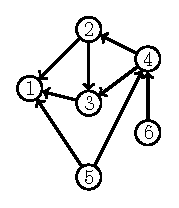
\includegraphics[width=0.15\textwidth]{acyclic}
	\caption{Acyclic graph.}
	\label{fig:acyclic}
	\bigskip
\end{figure}

Drawbacks of this type of measure are that it does not scale well for directed networks (asymmetric adjacency matrices) where it is not always possible to compute a unique, real leading eigenvector. Or, even worse, it is not applicable in acyclic networks. Figure \ref{fig:acyclic} illustrates how node $1$ in that network has only in-going edges and hence will have eigenvector zero centrality, according to (\ref{eqn:eigc}). Node $3$ has an out-going edge and two in-going edges, but the in-going one is incident on node $1$, and hence node $3$ will also have zero centrality. Following this argument for the remainder nodes, the result is a zero centrality for the whole network. To address these problems, variants based on Eigenvector Centrality such as PageRank and Katz centrality were developed.

\subsection*{PageRank and Katz Centrality}
In the task of finding the most important nodes in a network, two of the most widely used methods are PageRank and Katz Centrality. To solve Eigenvector Centrality problems in networks that do not have strongly connected components of more than one node resulting in a zero centrality vector, the main idea of these two methods is to give each node a small amount of centrality for free. 

Let $\mathbf{A}\in\mathbb{R}^{N\times N}$ be the adjacency matrix for a static network of $N$ nodes. Then, from (\ref{eqn:eigc}) PageRank Centrality is defined as

\begin{equation}
\label{eqn:pr1}
    x_i= \alpha\sum_{j=1}^{N}A_{ij}\frac{x_j}{k_j^{\text{out}}} + \beta,
\end{equation}
where $\alpha$, $\beta$ are positive parameters and $k_j^{\text{out}}$ denotes the out-degree of node $j$, i.e., the number of out-going links from that node. The first term correspond to the Eigenvector Centrality and the second term is the “free” part, the constant extra amount that all nodes receive. By including this additional component, we make sure that nodes with no incoming connections still receive centrality, and once they have a non-zero centrality score, they can distribute it to the other nodes they are linked to. This results in nodes that are connected to many others having a high centrality, regardless of whether they are part of a strongly connected component or an out-component.

The difference between PageRank and Katz centrality resides precisily in the way they spread the centrality over the network. In mathematical terms, Katz Centrality is obtained from (\ref{eqn:pr1}) when $k_j^{\text{out}}=1$ for each $j$,

\begin{equation}
\label{eqn:katz1}
    x_i= \alpha\sum_{j=1}^{N}A_{ij}x_j + \beta
\end{equation}

If a node with a high Katz score has links to many other nodes, then all of those linked nodes will also receive a high centrality score. PageRank, instead, is a variant in which the centrality derived from network neighbors is proportional to their centrality divided by their out-degree. Therefore, nodes that point to many others pass only a small amount of centrality on to each of those others, even if their own centrality is high.

By convenience, we set $k_j^{\text{out}}=1$ in (\ref{eqn:pr1}) to avoid zero-division for nodes with no outgoing edges. Thus, we can express PageRank Centrality in matrix form as

\begin{equation}
\label{eqn:pr2}
    \mathbf{x} = \alpha\mathbf{AD}^{-1}\mathbf{x} + \beta \mathbf{1},
\end{equation}
with $\mathbf{1}$ being the vector of ones $(1,\dots,1)$ and $\mathbf{D}$ being the diagonal matrix with elements $D_{ii} = max(k_i^{\text{out}},1)$. Rearranging for $\mathbf{x}$ and setting the conventional value of $\beta=1$, the PageRank centrality yields

\begin{equation}
\label{eqn:pr3}
    \mathbf{x} = (\mathbf{I} - \alpha\mathbf{AD}^{-1})^{-1} \mathbf{1}.
\end{equation}
Again, a similar expression for Katz Centrality is obtained if we consider $\mathbf{D}^{-1}= \mathbf{I}$, for $\mathbf{I}$ denoting the identity matrix of order $N$.

We seek $\alpha$ such that $(\mathbf{I}-\alpha\mathbf{AD}^{-1})^{-1}$ does not diverges, i.e. $\text{det}(\mathbf{I}-\alpha\mathbf{AD}^{-1})\neq 0$, or what is the same, $\text{det}(\mathbf{AD}^{-1}-\alpha^{-1}\mathbf{I})\neq 0$, that it is simply the characteristic equation whose roots $\alpha^{-1}$ are equal to the eigenvalues of the adjacency matrix. The first value of $\alpha$ that makes this determinant $0$ is $\alpha^{-1}=\lambda_1$ so this suggests a good value for $\alpha$ bounded by $0 < \alpha < 1/\lambda_1 $, being $\lambda_1$ the largest eigenvalue of $\mathbf{AD}^{-1}$ (Google uses $\alpha = 0.85$). In the choice of $\alpha$ we must take into account that the closer we are to the largest eigenvalue the maximum amount of weight on the eigenvector term will be place and the smallest amount on the constant term. If we let instead $\alpha\to 0$, then only the constant term will survive in Eq. (\ref{eqn:katz1}) resulting in all nodes with equal centrality.

PageRank was developed by Google co-founders Larry Page and Sergey Brin as a way to rank websites in their search engine results. The basic idea behind PageRank is that a node is considered important if it is linked to by many other important nodes. The PageRank score of a node is determined by the sum of the PageRank scores of the nodes that link to it, with a damping factor applied to reduce the influence of nodes with many outbound links. 

PageRank and Katz Centrality are widely used in the field of network analysis and has been applied to a wide range of networks, including the World Wide Web, social networks, or biological networks \cite{brin1998anatomy,jeong2001lethality,wasserman1994social}. Overall, each centrality measure provides a different perspective on the importance of a node in a network (see Figure \ref{centrality}) and can be useful in various applications, such as network analysis, recommendation systems, or identifying key players in complex systems. The most appropriate centrality measure will require a more detailed analysis of the specific characteristics of the network in question.

Katz Centrality is covered to a greater extent in the next section \ref{sec:back} as it is the central topic of this thesis.

\begin{figure}[h]\centering
	\includegraphics[width=1.0\textwidth]{centrality_plots}
	\caption{Examples of A) Degree Centrality, B) Betweenness Centrality, C) Closeness Centrality, D) Eigenvector Centrality, E) Katz Centrality and F) PageRank from Zachary’s Karate Club graph dataset \cite{zachary1977information}.}
	\label{centrality}
	\bigskip
\end{figure}

\section{Background on Katz Centrality in static networks}
\label{sec:back}

Katz Centrality was first introduced by Leo Katz \cite{katz1953new} in 1953 as a way to measure the relative importance of nodes in a network based on the number of paths that pass through them. This measure is obtained by assigning a score to each node in the network based on the sum of the scores of all nodes that are one step away from it, plus a fraction of the scores of all nodes that are two steps away, and so on, up to an arbitrary limit or threshold.

Expression (\ref{eqn:pr3}) for Katz Centrality can be rewritten using Neumann series, as a generalization of geometric series, by

\begin{equation}
\label{eqn:katz2}
    \mathbf{x}=(\mathbf{I}-\alpha\mathbf{A})^{-1}\mathbf{1}=\left(\sum_{k=0}^{\infty}\alpha^k \mathbf{A}^k\right)\mathbf{1},
\end{equation}
giving a practical expansion to compute by approximation/truncation the \textit{resolvent of the adjacency matrix} 

\begin{equation}
\label{eqn:katz3}
    (\mathbf{I}-\alpha\mathbf{A})^{-1} = \mathbf{I} + \alpha\mathbf{A} + \alpha^2\mathbf{A}^2 + \cdots + \alpha^k\mathbf{A}^k + \cdots
\end{equation}
which converges for $\alpha<1/\rho(A)$ where $\rho(\cdot)$ denotes the spectral radius. 

This series is in fact the original form of centrality conceived by Leo Katz, who considered for each node $i$ the influence of all the nodes connected by a $k$-length walk to $i$ with no restriction in reuse of nodes and edges. Thus, $\alpha$ can be considered an attenuation parameter as the probability that an edge is successfully traversed, penalizing those nodes furthest away from $i$. 

Considering messages being passed along the directed edges, one important consequence of the above expansion is that elements of the resolvent matrix can be considered as a measure of the ability for a node $i$ to pass information to $j$ taking into account all possible routes, with longer ones given less importance. In that sense, if we consider row sums in the resolvent matrix as a linear combination of powers of $\mathbf{A}$ we can talk about the \textit{broadcast centrality vector} ($\mathbf{b}$) as the ability to send information for each node in the network 

\begin{equation}
\label{eqn:broad}
    \mathbf{b}=(\mathbf{I}-\alpha\mathbf{A})^{-1} \mathbf{1}.
\end{equation}
Similarly, the column sums of the resolvent matrix give a notion of the ability to receive information which is defined as the \textit{receive centrality vector} ($\mathbf{r}$) of the network

\begin{equation}
\label{eqn:receiv}
    \mathbf{r} = (\mathbf{I}-\alpha\mathbf{A})^{-T} \mathbf{1}.
\end{equation}
Broadly speaking, a node with a high Katz broadcast centrality will be an effective starting point for spreading a rumor, and a node with high Katz receive centrality will be an ideal location to receive the latest rumor.

Overall, Katz centrality is a widely used centrality measure, for both directed and undirected networks, because it provides a nuanced and flexible way to assess the importance of nodes in a network based on their position in the network and their potential for information flow and communication.

\section{Motivation of the study}
\label{sec:motiv}
Dynamic networks, or what is the same, systems involving transient interactions are commonly found in real problems across various fields. Currently, the most popular approach is to examine network activity over discrete time frames or snapshots and analyze network status at these time slices. This method presents a number of challenges when it comes to modeling and computing, as it fails to account for the time-sensitive nature of network connections. If the time frame is too large, the ability to reproduce high-frequency transient behaviour, where an edge switches on and off multiple times in the space of a single window, is lost. On the other hand, if it is too narrow, it could result in a large number of empty time frames that can lead to redundant processes, wasting computational effort. Additionally, when time windows are too finely spaced, a static model may give a false impression of accuracy since it is not able to reflect altogether the time at which instantaneous information is sent, then received and later processed in time, as happens in many human communication media, with the subsequent loss of information in the network.

Therefore, to address these limitations the present work analyzes a continuous-time framework developed in \cite{grindrod2014dynamical} that can directly extract centrality information from a network's time-dependent adjacency matrix. This new centrality system expands the concept of the well-known Katz measure and allows us to identify and monitor the most influential nodes in dynamic networks over time at any level of detail in a natural and efficient way.

% ---------------------------------------------------------------------
% ---------------------------------------------------------------------
